%
% dreieck3d2.tex
%
% (c) 2021 Prof Dr Andreas Müller, OST Ostschweizer Fachhochschule
%
\documentclass[tikz]{standalone}
\usepackage{times}
\usepackage{amsmath}
\usepackage{txfonts}
\usepackage[utf8]{inputenc}
\usepackage{graphics}
\usetikzlibrary{arrows,intersections,math}
\usepackage{ifthen}
\begin{document}

\newboolean{showgrid}
\setboolean{showgrid}{false}
\def\breite{4}
\def\hoehe{4}

\begin{tikzpicture}[>=latex,thick]

% Povray Bild
\node at (0,0) {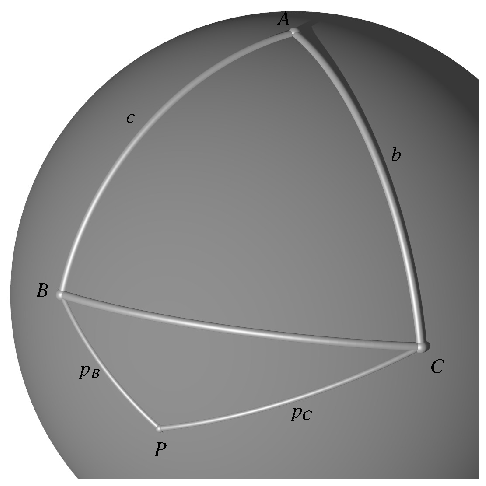
\includegraphics[width=8cm]{dreieck3d2.jpg}};

% Gitter
\ifthenelse{\boolean{showgrid}}{
\draw[step=0.1,line width=0.1pt] (-\breite,-\hoehe) grid (\breite, \hoehe);
\draw[step=0.5,line width=0.4pt] (-\breite,-\hoehe) grid (\breite, \hoehe);
\draw                            (-\breite,-\hoehe) grid (\breite, \hoehe);
\fill (0,0) circle[radius=0.05];
}{}

\node at (0.7,3.8) {$A$};
\node at (-3.4,-0.8) {$B$};
\node at (3.3,-2.1) {$C$};
\node at (-1.4,-3.5) {$P$};

\node at (-1.9,2.1) {$c$};
%\node at (-0.2,-1.2) {$a$};
\node at (2.6,1.5) {$b$};

\node at (-2.6,-2.2) {$p_b$};
\node at (1,-2.9) {$p_c$};

%\node at (0.7,3) {$\alpha$};
%\node at (-2.5,-0.5) {$\beta$};
%\node at (2.3,-1.2) {$\gamma$};

\end{tikzpicture}

\end{document}

